\newtheorem{defn}{Definition}
\begin{frame}[fragile]{Metric spaces encode structure}
\centering
\resizebox{!}{4.5cm}{
\begin{tikzpicture}[dot/.style={circle,inner sep=2pt,fill,name=#1},
    extended line/.style={shorten >=-#1,shorten <=-#1},
    extended line/.default=1cm]

% draw the grid
\uncover<1-2> {
    \draw[->] (0,-0.25) -- (0,5.25) ;
    \draw[->] (-0.25,0) -- (5.25,0) ;
    \foreach \i in {1,...,5} {
        \draw[dotted] (-0.25,\i) -- (5.25,\i);
        \draw[dotted] (\i,-0.25) -- (\i,5.25);
    }
}

% draw the points
\uncover<1-2> {
    \node [dot=a,label=above left:a] at (1,1) {};
    \node [dot=b,label=above:b] at (2,4) {};
    \node [dot=c,label=above right:c] at (4,2) {};
}

% draw the L2 metric
\uncover<1> {
    \draw (a) -- (b) -- (c) -- (a);
    \node at (3,1.25) {$\sqrt{10}$};
    \node at (1,2.75) {$\sqrt{10}$};
    \node at (3.5,3.25) {$2\sqrt{2}$};
    \node at (8, 4.5) {
        Euclidean distance:
        };
    \node at (9,2.5) {

        $\begin{aligned}
        {X}& = \mathbb{R}^p \\
        \displaystyle
        d(x,y)
        &=
        \ltwo{x-y}
        &=
        \displaystyle
        \left(\sum_{i=1}^p (x_i-y_i)^2\right)^{\frac 1 2} \\
        \end{aligned}$
        };
    %\node at (9, 0.5) { Runtime to calculate distance: $O(p)$ };
}

% draw the L1 metric
\uncover<2> {
    \draw (a) -- (1,4) -- (b) -- (4,4) -- (c) -- (4,1) -- (a);
    \node at (2.5,1.25) {$4$};
    \node at (1.25,2.75) {$4$};
    \node at (3.5,3.5) {$4$};
    \node at (9, 4.5) {
        $L_1$ (Manhattan, taxicab) distance:
        };
    \node at (9,2.5) {
        $\begin{aligned}
        {X}& = \mathbb{R}^p \\
        \displaystyle
        d(x,y)
        &=
            \lone{x-y}
        =
        \displaystyle
        \sum_{i=1}^p |x_i-y_i| \\
        \end{aligned}$
        };
    %\node at (9, 0.5) { Runtime to calculate distance: $O(p)$ };
}

\uncover<3-> {
    %\node[anchor=west] at (0,5) {Easy to define a metric from the class hierarchy/confusion matrix};
    \node at (1,2) {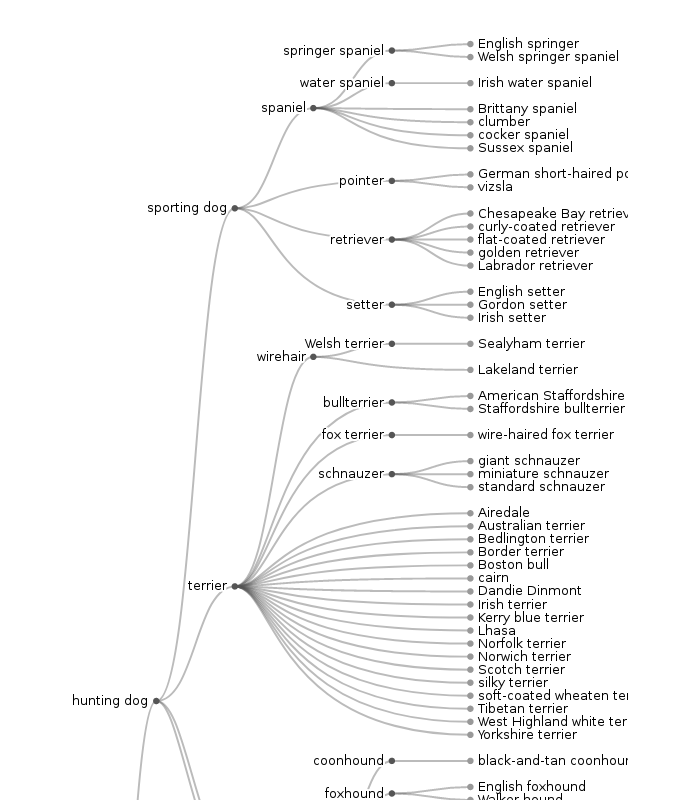
\includegraphics[height=1.8in]{img/imagent-hierarchy}};
    \node at (8,2) {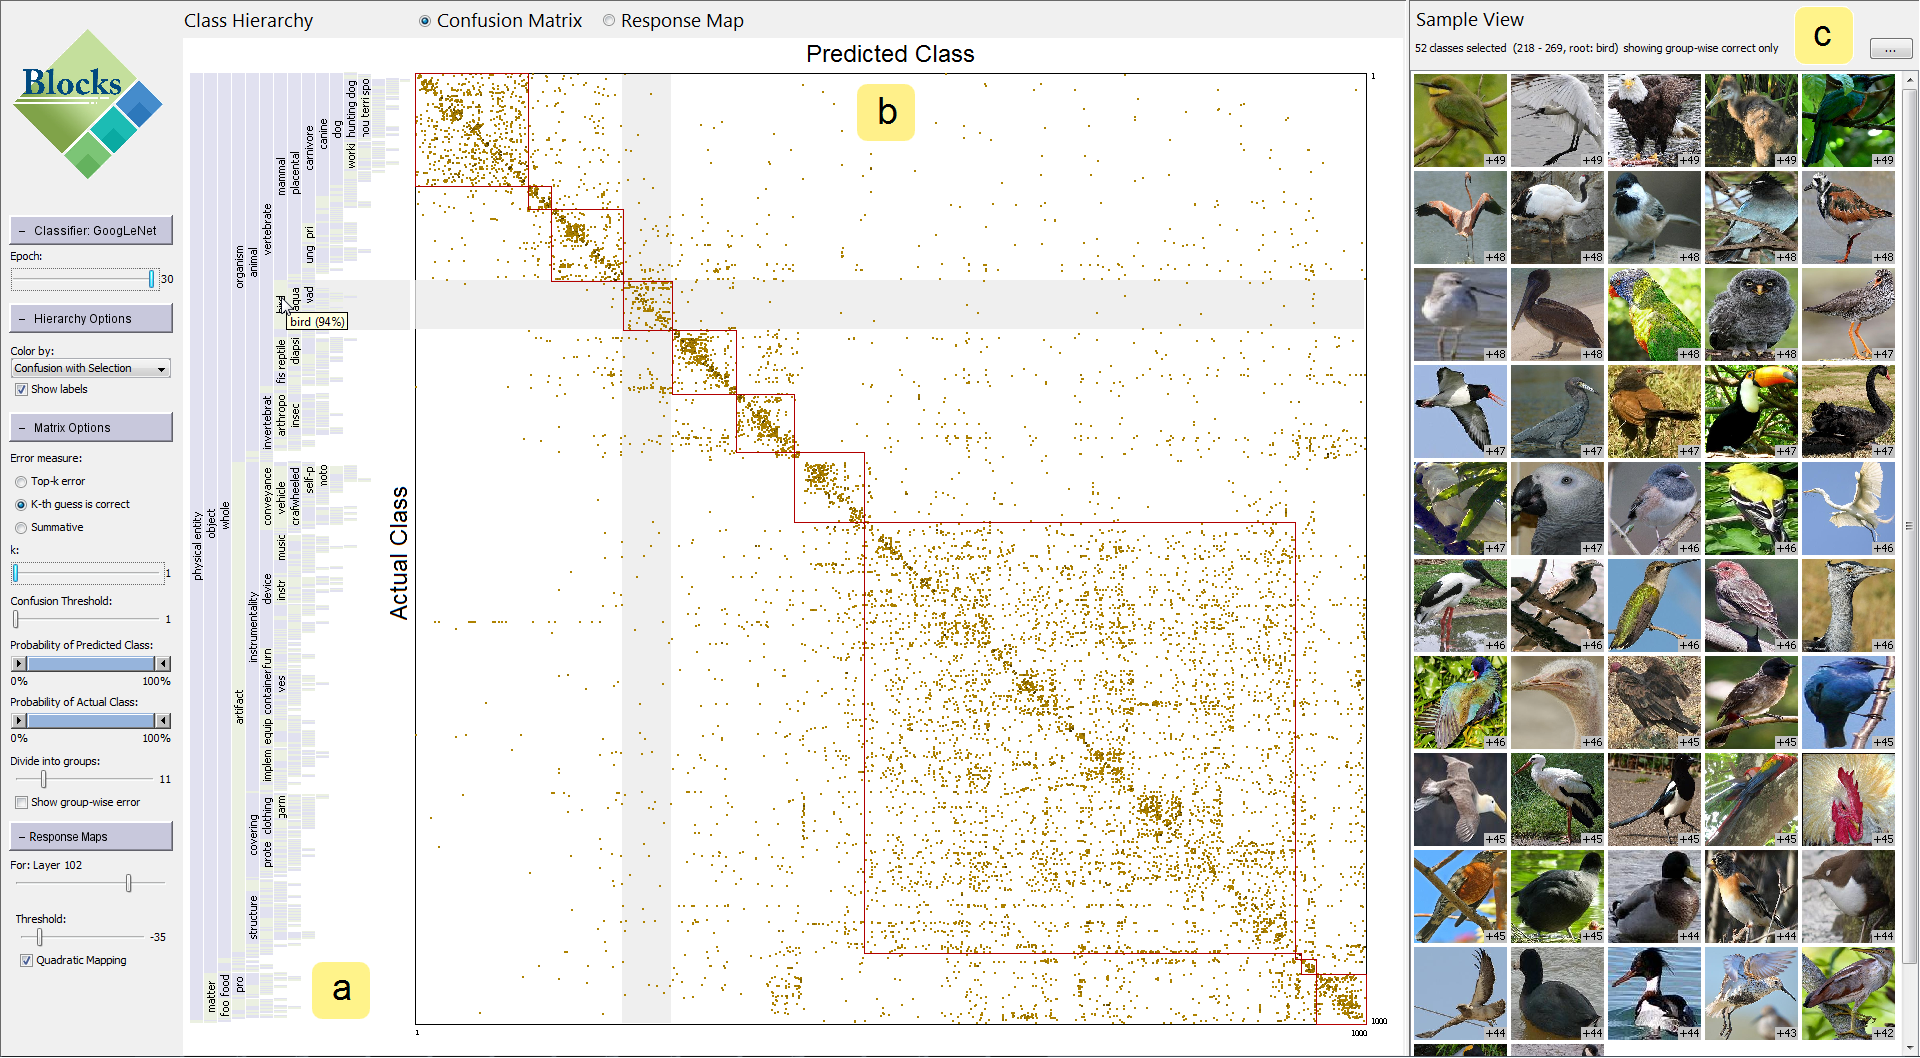
\includegraphics[height=1.8in]{img/teaser}};
}

%\uncover<3> {
    %\node at (0,0) {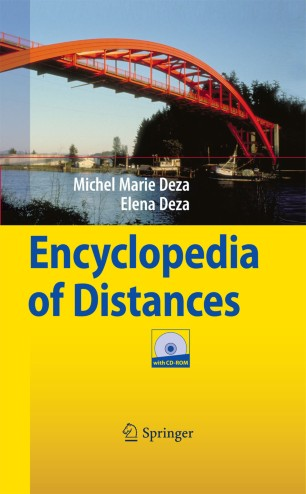
\includegraphics[height=3in]{img/encyclopedia}};
%}

% draw the Linf metric
%\uncover<3> {
    %\draw (a) -- (1,4);
    %\draw (4,4) -- (c);
    %\draw (a) -- (4,1);
    %\node at (2.5,1.25) {$3$};
    %\node at (1.25,2.75) {$3$};
    %\node at (3.5,3.5) {$2$};
    %\node at (8, 4.5) {
        %$L_\infty$ (sup) distance:
        %};
    %\node at (9,2.5) {
        %$\begin{aligned}
        %{X}& = \mathbb{R}^p \\
        %\displaystyle
        %d(x,y)
        %&=
        %\displaystyle
        %\sup_{i\in\{1..p\}} |x_i-y_i| \\
        %\end{aligned}$
        %};
    %\node at (9, 0.5) { Runtime to calculate distance: $O(p)$ };
%}

%% draw the Lebesgue metric
%\uncover<4> {
    %\node at (9, 4.5) {
        %Lebesgue family of distances:
        %};
    %\node at (9,2.5) {
        %$\begin{aligned}
        %{X}& = \mathbb{R}^n \\
        %\displaystyle
        %d(x,y)
        %&=
        %\displaystyle
        %\left(\sum_{i\in\{1..n\}} |x_i-y_i|^n\right)^{\frac 1 n} \\
        %\end{aligned}$
        %};
    %\node at (9, 0.5) { Runtime to calculate distance: $O(n)$ };
%}

%% graph distances
%\uncover <6-7> {
    %\draw[color=red,line width=2pt] (3.35,3.1) -- (3.65,3.4);
    %\node[color=red] at (4,3.25) {\textbf{1?}};
%}
%\uncover<6> {
    %\draw[color=red,line width=2pt] (6,0) -- (12,5);
%}

%\uncover<5-6> {
    %\draw (a) -- (b) -- (c) -- (a);
    %\node at (3,1.25) {$2$};
    %\node at (1,2.75) {$4$};
    %\node at (3.5,3.25) {$5$};
    %\node at (9, 4.5) {
        %weighted, fully-connected graph distance
        %};
    %\node at (9,2.5) {
        %$\begin{aligned}
        %{X}& = \{a,b,c\} \\
        %\displaystyle
        %d(x,y)
        %&=
        %\text{edge weight}
        %\end{aligned}$
        %};
    %\node at (9, 0.5) { Runtime to calculate distance: $O(1)$ };
%}

%% graph distances
%\uncover<7> {
    %\draw (a) -- (b) -- (c) -- (a);
    %\node at (3,1.25) {$2$};
    %\node at (1,2.75) {$4$};
    %\node at (3.5,3.25) {$5$};
    %\node at (9, 4.5) {
        %Dijkstra graph distance
        %};
    %\node at (9,2.5) {
        %$\begin{aligned}
        %{X}& = \{a,b,c\} \\
        %\displaystyle
        %d(x,y)
        %&=
        %\text{shortest path between $x$ and $y$}
        %\end{aligned}$
        %};
    %\node at (9, 0.5) { Runtime to calculate distance: $O(e+v\log v)$ };
%}

%% graph distances
%\uncover<8> {
    %\draw (a) -- (b);
    %\draw (c) -- (a);
    %\node at (3,1.25) {$2$};
    %\node at (1,2.75) {$4$};
    %\node at (9, 4.5) {
        %Dijkstra graph distance
        %};
    %\node at (9,2.5) {
        %$\begin{aligned}
        %{X}& = \{a,b,c\} \\
        %\displaystyle
        %d(x,y)
        %&=
        %\text{shortest path between $x$ and $y$}
        %\end{aligned}$
        %};
    %\node at (9, 0.5) { Runtime to calculate distance: $O(e+v\log v)$ };
%}

%% graph distances
%\uncover<9> {
    %\draw (a) -- (b);
    %\node at (1,2.75) {$4$};
    %\node at (9, 4.5) {
        %Dijkstra graph distance
        %};
    %\node at (9,2.5) {
        %$\begin{aligned}
        %{X}& = \{a,b,c\} \\
        %\displaystyle
        %d(x,y)
        %&=
        %\text{shortest path between $x$ and $y$}
        %\end{aligned}$
        %};
    %\node at (9, 0.5) { Runtime to calculate distance: $O(e+v\log v)$ };
%}

%% graph distances
%\uncover<10> {
    %\node at (8, 4.5) {
        %trivial distance
        %};
    %\node at (9,2.5) {
        %$\begin{aligned}
        %{X}& = \{a,b,c\} \\
        %\displaystyle
        %d(x,y)
        %&=
        %\infty
        %\end{aligned}$
        %};
    %\node at (9, 0.5) { Runtime to calculate distance: $O(1)$ };
%}

%% graph distances
%\uncover<11> {
    %\node at (1,3) {
        %$d \left(
        %\text{
        %\begin{tikzpicture}
        %\node at (0,2) {};
        %\node [dot= ] at (1,1) {};
        %\node [dot= ] at (1,0) {};
        %\node [dot= ] at (0,1) {};
        %\draw (1,1) -- (1,0) -- (0,1) -- (1,1);
        %\end{tikzpicture}
        %,
        %\begin{tikzpicture}
        %\node at (0,2) {};
        %\node [dot= ] at (1,1) {};
        %\node [dot= ] at (1,0) {};
        %\node [dot= ] at (0,1) {};
        %\node [dot= ] at (0,0) {};
        %\draw (1,1) -- (1,0) -- (0,1) -- (1,1) -- (0,0) -- (0,1) -- (1,0) -- (0,0);
        %\end{tikzpicture}
        %}
        %\right)$
    %};
    %\node at (9, 4.5) {
        %\emph{graph metrics} are distances between graphs
        %};
    %\node at (9,2.5) {
        %$\begin{aligned}
        %{X}& = \text{set of all graphs} \\
        %\displaystyle
        %d(x,y)
        %&=
        %\text{many possibilities}
        %\end{aligned}$
        %};
    %\node at (9, 0.5) { Runtime to calculate distance: $O(1)$ };
%}

\end{tikzpicture}
}
\begin{defn}
A \emph{metric space} is a set ${X}$ equiped with a distance function $d : {X} \times {X} \rightarrow \mathbb{R}$ such that:
\begin{center}
\begin{tabular}{ll}
$d(x,y) \ge 0$ & $d(x,y) = 0$ iff $x=y$ \\
$d(x,y) = d(y,x)$ & $d(x,z) \le d(x,y) + d(y,z)$ \\
\end{tabular}
\end{center}
\end{defn}

\uncover<4>{
\vspace{-3.2in}
\begin{center}
\setlength{\fboxsep}{0pt}%
\setlength{\fboxrule}{1pt}%
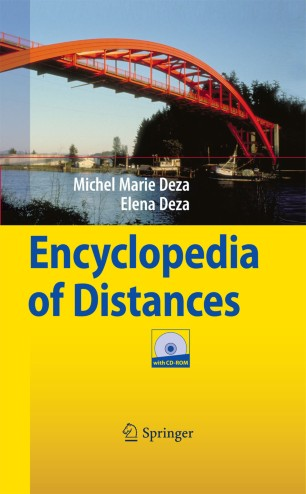
\includegraphics[height=3in]{img/encyclopedia}
\end{center}
}
\end{frame}


